\documentclass[11pt,a4paper]{report}
\usepackage[textwidth=37em,vmargin=30mm]{geometry}
\usepackage{calc,xunicode,amsmath,amssymb,paralist,enumitem,tabu,booktabs,datetime2,xeCJK,xeCJKfntef,listings}
\usepackage{tocloft,fancyhdr,tcolorbox,xcolor,graphicx,eso-pic,xltxtra,xelatexemoji}

\newcommand{\envyear}[0]{2025}
\newcommand{\envdatestr}[0]{2025-10-17}
\newcommand{\envfinaldir}[0]{webdb/2025/20251017/final}

\usepackage[hidelinks]{hyperref}
\hypersetup{
    colorlinks=false,
    pdfpagemode=FullScreen,
    pdftitle={Web Digest - \envdatestr}
}

\setlength{\cftbeforechapskip}{10pt}
\renewcommand{\cftchapfont}{\rmfamily\bfseries\large\raggedright}
\setlength{\cftbeforesecskip}{2pt}
\renewcommand{\cftsecfont}{\sffamily\small\raggedright}

\setdefaultleftmargin{2em}{2em}{1em}{1em}{1em}{1em}

\usepackage{xeCJK,xeCJKfntef}
\xeCJKsetup{PunctStyle=plain,RubberPunctSkip=false,CJKglue=\strut\hskip 0pt plus 0.1em minus 0.05em,CJKecglue=\strut\hskip 0.22em plus 0.2em}
\XeTeXlinebreaklocale "zh"
\XeTeXlinebreakskip = 0pt


\setmainfont{Brygada 1918}
\setromanfont{Brygada 1918}
\setsansfont{IBM Plex Sans}
\setmonofont{JetBrains Mono NL}
\setCJKmainfont{Noto Serif CJK SC}
\setCJKromanfont{Noto Serif CJK SC}
\setCJKsansfont{Noto Sans CJK SC}
\setCJKmonofont{Noto Sans CJK SC}

\setlength{\parindent}{0pt}
\setlength{\parskip}{8pt}
\linespread{1.15}

\lstset{
	basicstyle=\ttfamily\footnotesize,
	numbersep=5pt,
	backgroundcolor=\color{black!5},
	showspaces=false,
	showstringspaces=false,
	showtabs=false,
	tabsize=2,
	captionpos=b,
	breaklines=true,
	breakatwhitespace=true,
	breakautoindent=true,
	linewidth=\textwidth
}






\newcommand{\coverpic}[2]{
    % argv: itemurl, authorname
    Cover photo by #2~~(\href{#1}{#1})
}
\newcommand{\makeheader}[0]{
    \begin{titlepage}
        % \newgeometry{hmargin=15mm,tmargin=21mm,bmargin=12mm}
        \begin{center}
            
            \rmfamily\scshape
            \fontspec{BaskervilleF}
            \fontspec{Old Standard}
            \fontsize{59pt}{70pt}\selectfont
            WEB\hfill DIGEST
            
            \vfill
            % \vskip 30pt
            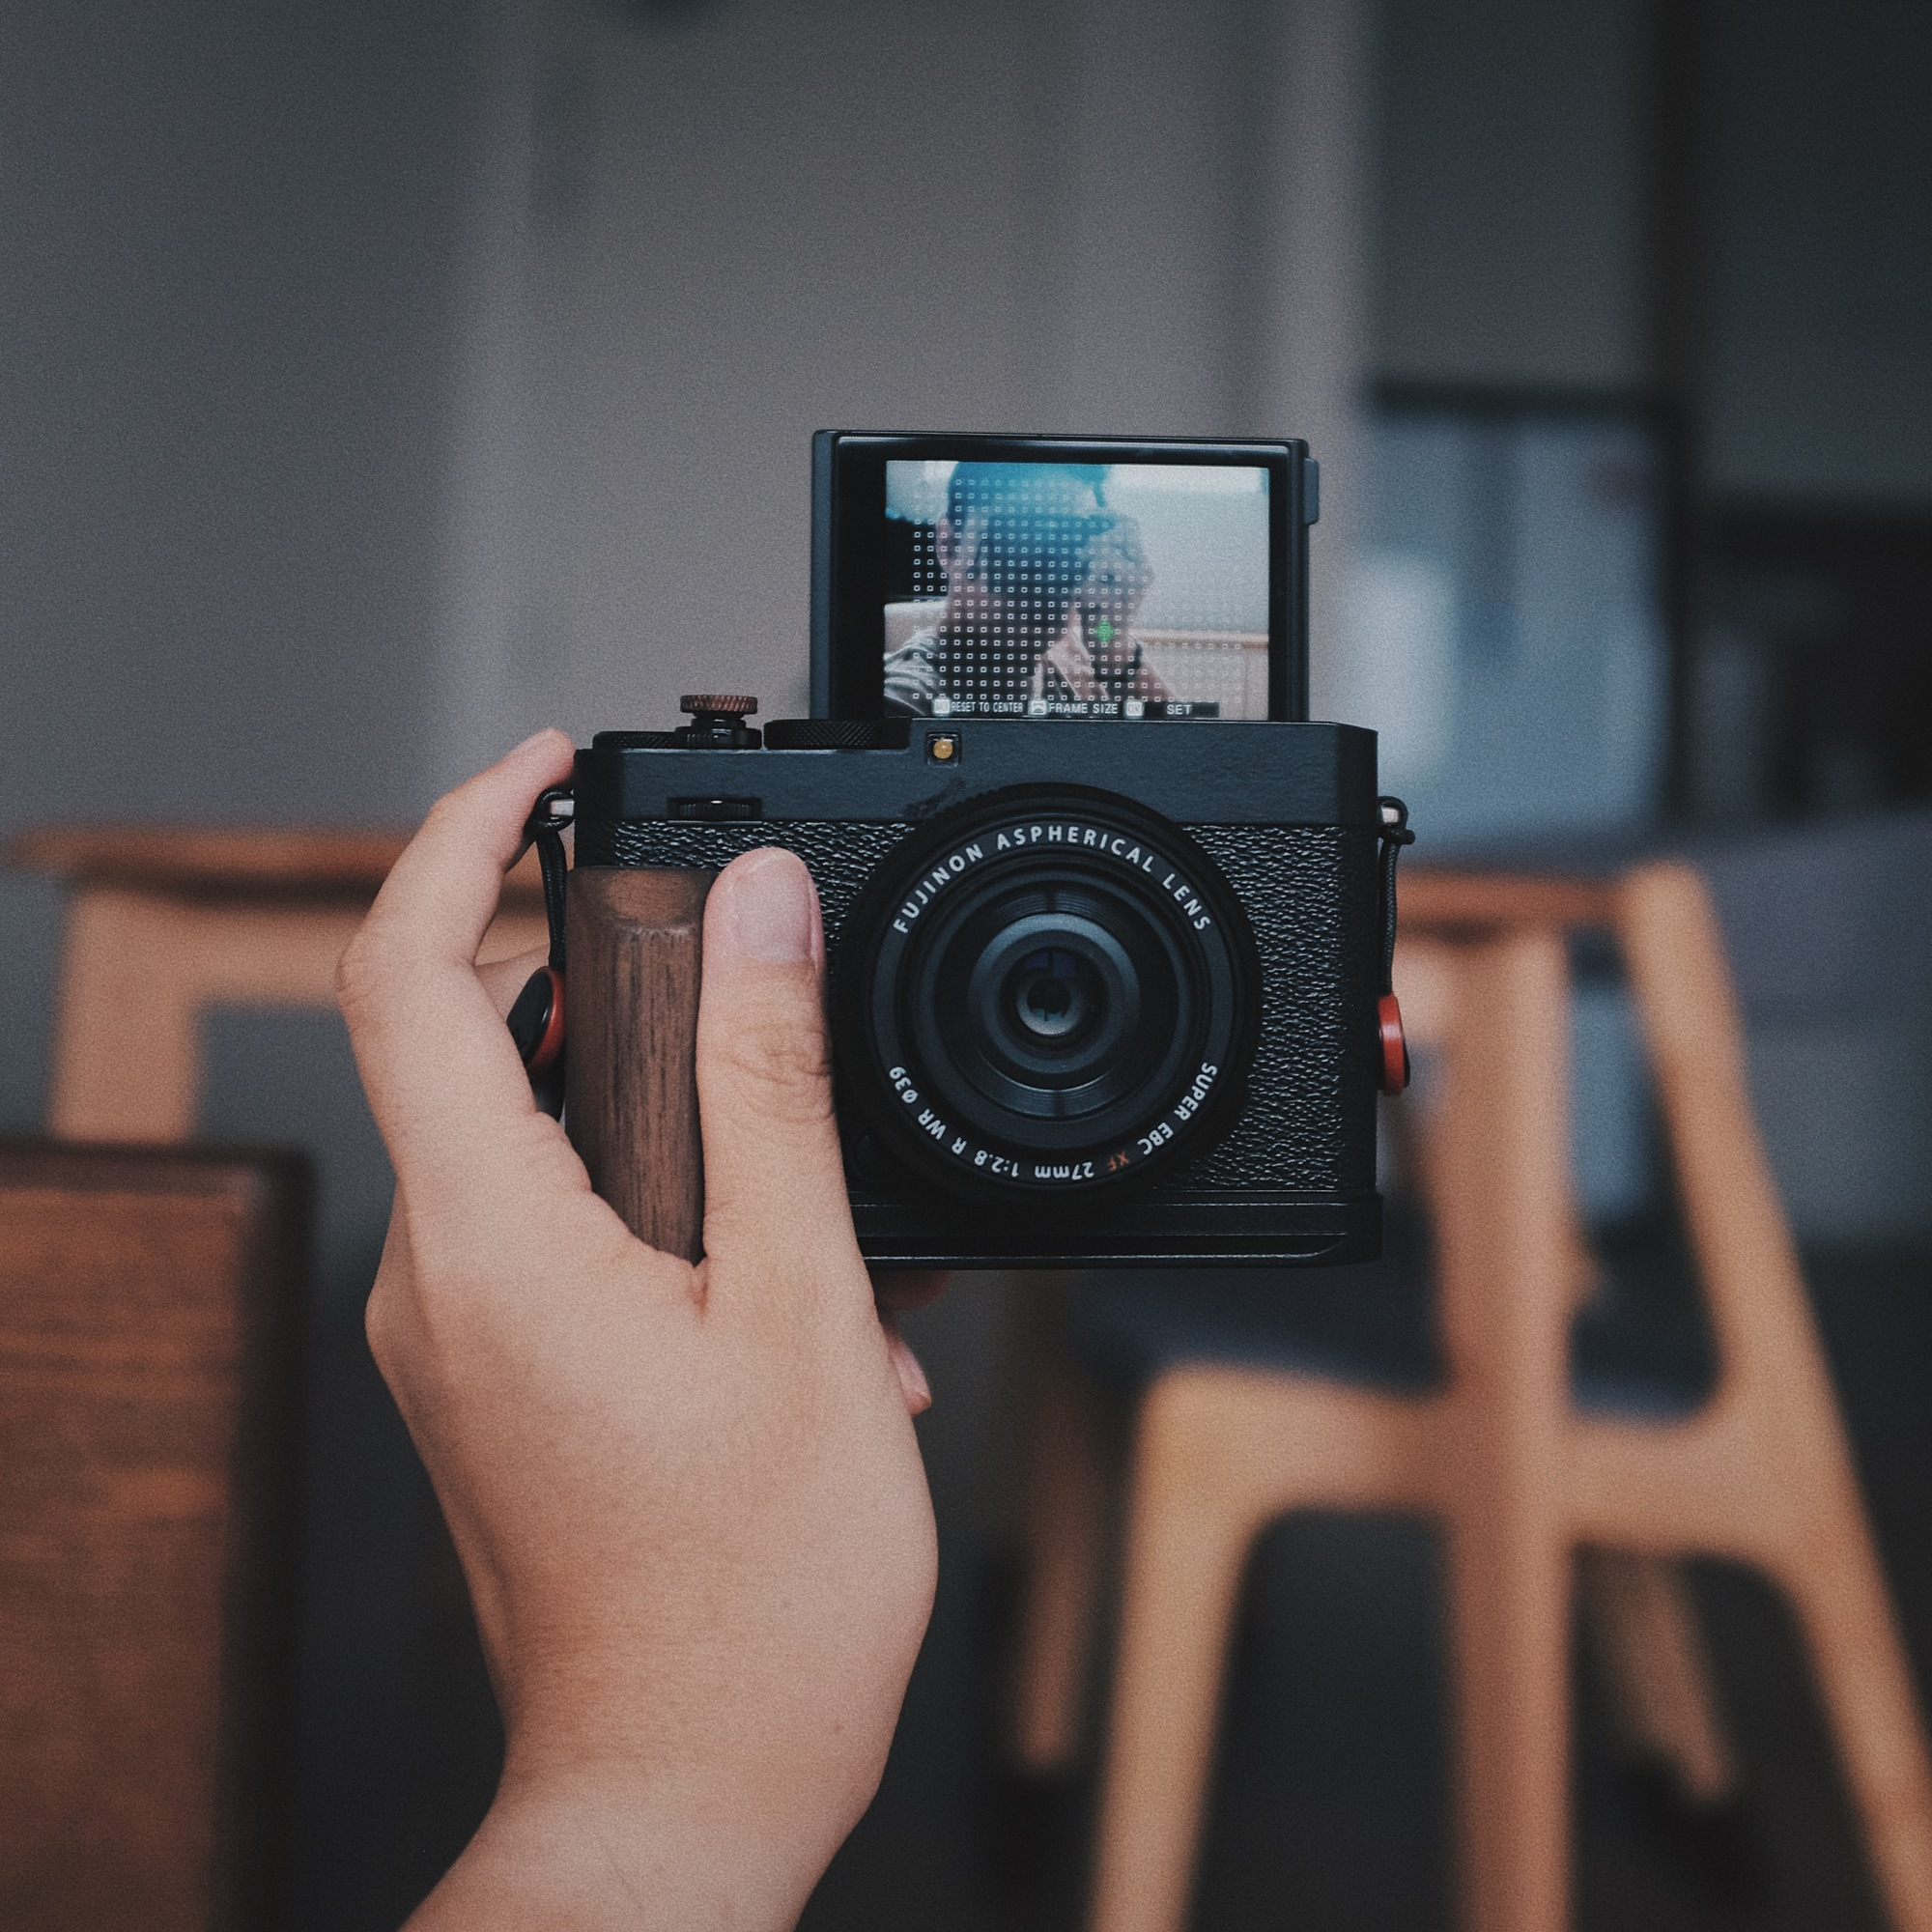
\includegraphics[width=\linewidth]{\envfinaldir/coverpic-prod.jpg}\par
            % \vskip 30pt
            \vfill

            \normalsize\rmfamily\scshape
            \copyright{} The Web Digest Project \hfill\large \envdatestr
        \end{center}
    \end{titlepage}
    % \restoregeometry
}
\newcommand{\simplehref}[1]{%
    \textcolor{blue!80!green}{\href{#1}{#1}}%
}
\renewcommand{\contentsname}{\center\Huge\sffamily\bfseries Contents\par\vskip 20pt}
\newcounter{ipartcounter}
\setcounter{ipartcounter}{0}
\newcommand{\ipart}[1]{
    % \vskip 20pt
    \clearpage
    \stepcounter{ipartcounter}
    \phantomsection
    \addcontentsline{toc}{chapter}{#1}
    % \begin{center}
    %     \Huge
    %     \sffamily\bfseries
    %     #1
    % \end{center}
    % \vskip 20pt plus 7pt
}
\newcounter{ichaptercounter}
\setcounter{ichaptercounter}{0}
\newcommand{\ichapter}[1]{
    % \vskip 20pt
    \clearpage
    \stepcounter{ichaptercounter}
    \phantomsection
    \addcontentsline{toc}{section}{\numberline{\arabic{ichaptercounter}}#1}
    \begin{center}
        \Huge
        \sffamily\bfseries
        #1
    \end{center}
    \vskip 20pt plus 7pt
}
\newcommand{\entrytitlefont}[1]{\subsection*{\raggedright\Large\sffamily\bfseries#1}}
\newcommand{\entryitemGeneric}[2]{
    % argv: title, url
    \parbox{\linewidth}{
        \entrytitlefont{#1}\par\vskip 5pt
        \footnotesize\ttfamily\mdseries
        \simplehref{#2}
    }\vskip 11pt plus 11pt minus 1pt
}
\newcommand{\entryitemGithub}[3]{
    % argv: title, url, desc
    \parbox{\linewidth}{
        \entrytitlefont{#1}\par\vskip 5pt
        \footnotesize\ttfamily\mdseries
        \simplehref{#2}\par\vskip 5pt
        \small\rmfamily\mdseries#3
    }\vskip 11pt plus 11pt minus 1pt
}
\newcommand{\entryitemAp}[3]{
    % argv: title, url, desc
    \parbox{\linewidth}{
        \entrytitlefont{#1}\par\vskip 5pt
        \footnotesize\ttfamily\mdseries
        \simplehref{#2}\par\vskip 5pt
        \small\rmfamily\mdseries#3
    }\vskip 11pt plus 11pt minus 1pt
}
\newcommand{\entryitemHackernews}[3]{
    % argv: title, hnurl, rawurl
    % \parbox{\linewidth}{
    %     \entrytitlefont{#1}\par\vskip 5pt
    %     \footnotesize\ttfamily\mdseries
    %     \simplehref{#3}\par
    %     \textcolor{black!50}{\href{#2}{#2}}
    % }\vskip 11pt plus 11pt minus 1pt
    \begin{minipage}{\linewidth}
            \entrytitlefont{#1}\par\vskip 5pt
            \footnotesize\ttfamily\mdseries
            \simplehref{#3}\par
            \textcolor{black!50}{\href{#2}{#2}}
    \end{minipage}\par\vskip 11pt plus 11pt minus 1pt
}







\begin{document}

\makeheader

\tableofcontents\clearpage




\ipart{Developers}
\ichapter{Hacker News}
\entryitemTwoLinks{How I bypassed Amazon's Kindle web DRM}{https://news.ycombinator.com/item?id=45610226}{https://blog.pixelmelt.dev/kindle-web-drm/}

\entryitemTwoLinks{A conspiracy to kill IE6 (2019)}{https://news.ycombinator.com/item?id=45608887}{https://blog.chriszacharias.com/a-conspiracy-to-kill-ie6}

\entryitemTwoLinks{test-ipv6.com will stay online}{https://news.ycombinator.com/item?id=45608795}{https://status.test-ipv6.com}

\entryitemTwoLinks{Mysterious Intrigue Around an x86 "Corporate Entity Other Than Intel/AMD"}{https://news.ycombinator.com/item?id=45608285}{https://www.phoronix.com/news/x86-Opcodes-Not-AMD-Or-Intel}

\entryitemTwoLinks{Gemini 3.0 spotted in the wild through A/B testing}{https://news.ycombinator.com/item?id=45607758}{https://ricklamers.io/posts/gemini-3-spotted-in-the-wild/}

\entryitemTwoLinks{Claude Skills}{https://news.ycombinator.com/item?id=45607117}{https://www.anthropic.com/news/skills}

\entryitemTwoLinks{Codex Is Live in Zed}{https://news.ycombinator.com/item?id=45606698}{https://zed.dev/blog/codex-is-live-in-zed}

\entryitemTwoLinks{Video game union workers rally against \$55B private acquisition of EA}{https://news.ycombinator.com/item?id=45606394}{https://www.eurogamer.net/ea-union-workers-rally-against-55bn-saudi-backed-private-acquisition-with-formal-petition-to-regulators}

\entryitemTwoLinks{How America got hooked on ultraprocessed foods}{https://news.ycombinator.com/item?id=45605921}{https://www.nytimes.com/interactive/2025/10/16/well/eat/ultraprocessed-food-junk-history.html}

\entryitemTwoLinks{Tor browser removing various Firefox AI features}{https://news.ycombinator.com/item?id=45605842}{https://blog.torproject.org/new-alpha-release-tor-browser-150a4/}

\entryitemTwoLinks{DoorDash and Waymo launch autonomous delivery service in Phoenix}{https://news.ycombinator.com/item?id=45605501}{https://about.doordash.com/en-us/news/waymo}

\entryitemTwoLinks{Why I Chose Elixir Phoenix over Rails, Laravel, and Next.js}{https://news.ycombinator.com/item?id=45605291}{https://akarshc.com/post/phoenix-for-my-project.html}

\entryitemTwoLinks{Lace: A New Kind of Cellular Automata Where Links Matter}{https://news.ycombinator.com/item?id=45605153}{https://www.novaspivack.com/science/introducing-lace-a-new-kind-of-cellular-automata}

\entryitemTwoLinks{Electricity can heal wounds three times as fast (2023)}{https://news.ycombinator.com/item?id=45604779}{https://www.chalmers.se/en/current/news/mc2-how-electricity-can-heal-wounds-three-times-as-fast/}

\entryitemTwoLinks{Hyperflask – Full stack Flask and Htmx framework}{https://news.ycombinator.com/item?id=45604673}{https://hyperflask.dev/}

\entryitemTwoLinks{European.cloud: A Curated Directory of EU-Based Cloud Providers}{https://news.ycombinator.com/item?id=45604672}{https://european.cloud/}

\entryitemTwoLinks{A stateful browser agent using self-healing DOM maps}{https://news.ycombinator.com/item?id=45604451}{https://100x.bot/a/a-stateful-browser-agent-using-self-healing-dom-maps}

\entryitemTwoLinks{Nightmare Fuel: Skibidi Toilet and the Monstrous Digital}{https://news.ycombinator.com/item?id=45604372}{https://journal.media-culture.org.au/index.php/mcjournal/article/view/3108}

\entryitemTwoLinks{Liquibase continues to advertise itself as "open source" despite license switch}{https://news.ycombinator.com/item?id=45602676}{https://github.com/liquibase/liquibase/issues/7374}

\entryitemTwoLinks{Elixir 1.19}{https://news.ycombinator.com/item?id=45602428}{https://elixir-lang.org/blog/2025/10/16/elixir-v1-19-0-released/}\ichapter{Phoronix}
\entryitemGeneric{\hskip 0pt{}Fedora 43 Is Not Ready For Release Next Week}{https://www.phoronix.com/news/Fedora-43-No-Go}

\entryitemGeneric{\hskip 0pt{}Meta Uncovers RDSEED Architectural Issue In AMD Zen 5 CPUs}{https://www.phoronix.com/news/AMD-EPYC-Turin-RDSEED-Bug}

\entryitemGeneric{\hskip 0pt{}Linux Affected By Decade Old Bug In Software RAID Around O\_DIRECT Usage}{https://www.phoronix.com/news/Linux-RAID-Bug-O-DIRECT}

\entryitemGeneric{\hskip 0pt{}Mysterious Intrigue Around An x86 "Corporate Entity Other Than Intel/AMD"}{https://www.phoronix.com/news/x86-Opcodes-Not-AMD-Or-Intel}

\entryitemGeneric{\hskip 0pt{}An Early Look At Linux 6.18 Performance With Intel Xeon 6 Granite Rapids}{https://www.phoronix.com/review/linux-618-intel-gnr}

\entryitemGeneric{\hskip 0pt{}AOMP 22.0-1 Brings Many Improvements For AMD's Fortran Compiler GPU Offloading}{https://www.phoronix.com/news/AMD-AOMP-22.0-1}

\entryitemGeneric{\hskip 0pt{}LLVM/Clang 22 Merges Support For Intel Nova Lake "-march=novalake"}{https://www.phoronix.com/news/LLVM-Clang-22-Nova-Lake}

\entryitemGeneric{\hskip 0pt{}Mesa NVK Lands Support For VK\_NVX\_image\_view\_handle - Needed For NVIDIA DLSS}{https://www.phoronix.com/news/Mesa-NVK-NVK-Image-Handle}

\entryitemGeneric{\hskip 0pt{}Latest Linux Patches For Homa Posted: TCP Alternative With 10~100x Lower Tail Latency}{https://www.phoronix.com/news/Linux-Homa-2025-Patches}


\ipart{Developers~~~~(zh-Hans)}
\ichapter{Solidot}
\entryitemGeneric{\hskip 0pt{}日本政府要求 OpenAI 停止侵权}{https://www.solidot.org/story?sid=82564}

\entryitemGeneric{\hskip 0pt{}苹果新 MacBook Pro 电池续航力长达 24 小时}{https://www.solidot.org/story?sid=82563}

\entryitemGeneric{\hskip 0pt{}到 2050 年全球气温可能上升 2C}{https://www.solidot.org/story?sid=82562}

\entryitemGeneric{\hskip 0pt{}美国近七成成年人肥胖}{https://www.solidot.org/story?sid=82561}

\entryitemGeneric{\hskip 0pt{}Reddit 联合创始人称大部分互联网已死}{https://www.solidot.org/story?sid=82560}

\entryitemGeneric{\hskip 0pt{}GLP-1 减肥药有治疗糖尿病的潜力}{https://www.solidot.org/story?sid=82559}

\entryitemGeneric{\hskip 0pt{}美国近四成 2 岁以下儿童接触智能手机}{https://www.solidot.org/story?sid=82558}

\entryitemGeneric{\hskip 0pt{}苹果承诺增加在华投资}{https://www.solidot.org/story?sid=82557}

\entryitemGeneric{\hskip 0pt{}Firefox 145 Beta 停止发布 32 位 Linux 版本}{https://www.solidot.org/story?sid=82556}

\entryitemGeneric{\hskip 0pt{}黑客入侵安全公司窃取未披露漏洞信息和源代码}{https://www.solidot.org/story?sid=82555}

\entryitemGeneric{\hskip 0pt{}Firefox 144.0 释出}{https://www.solidot.org/story?sid=82554}

\entryitemGeneric{\hskip 0pt{}青少年使用社媒与认知能力下降相关}{https://www.solidot.org/story?sid=82553}

\entryitemGeneric{\hskip 0pt{}美国扣押柬埔寨电诈集团价值 150 亿美元的比特币}{https://www.solidot.org/story?sid=82552}

\entryitemGeneric{\hskip 0pt{}FSF 宣布 Librephone 项目}{https://www.solidot.org/story?sid=82551}

\entryitemGeneric{\hskip 0pt{}研究发现卫星未加密传输敏感信息}{https://www.solidot.org/story?sid=82550}

\entryitemGeneric{\hskip 0pt{}商务部首次以 WPS 文档格式发表公告}{https://www.solidot.org/story?sid=82549}

\entryitemGeneric{\hskip 0pt{}女性被系统性的刻画成比男性更年轻}{https://www.solidot.org/story?sid=82548}

\entryitemGeneric{\hskip 0pt{}Google 限制 Android 侧载是其至今采取的最反消费者举措}{https://www.solidot.org/story?sid=82547}

\entryitemGeneric{\hskip 0pt{}NASA JPL 裁员 550 人}{https://www.solidot.org/story?sid=82546}

\entryitemGeneric{\hskip 0pt{}软件更新导致部分吉普牧马人 4xe 变砖}{https://www.solidot.org/story?sid=82545}\ichapter{V2EX}
\entryitemGeneric{\hskip 0pt{}[推广] 极客时间课程全场 5 折并且官方返现全部归还,盖楼送一门极客时间课程}{https://www.v2ex.com/t/1166273}

\entryitemGeneric{\hskip 0pt{}[问与答] 求推荐: iOS 上免费 好用的水印相机}{https://www.v2ex.com/t/1166270}

\entryitemGeneric{\hskip 0pt{}[问与答] Android lineageos 开启 clash 后,打开热点,无法上网。}{https://www.v2ex.com/t/1166269}

\entryitemGeneric{\hskip 0pt{}[生活] 我广西的老表现在沉迷新澳门那种彩票,怎么样告诉他不要沉迷?}{https://www.v2ex.com/t/1166268}

\entryitemGeneric{\hskip 0pt{}[前端开发] 关于 AI 助力脚本(Userscript)开发}{https://www.v2ex.com/t/1166267}

\entryitemGeneric{\hskip 0pt{}[职场话题] 大家公司写 Java /go 都用什么 IDE, 还用 IDEA 还是用 cursor 之类的?}{https://www.v2ex.com/t/1166266}

\entryitemGeneric{\hskip 0pt{}[Android] 选旗舰机还是折叠屏}{https://www.v2ex.com/t/1166265}

\entryitemGeneric{\hskip 0pt{}[分享创造] Veo3.1 上线,惊艳的电影级效果}{https://www.v2ex.com/t/1166264}

\entryitemGeneric{\hskip 0pt{}[生活] 老家父母会有让你在老家盖新房的执念么?}{https://www.v2ex.com/t/1166263}

\entryitemGeneric{\hskip 0pt{}[游戏] 为什么我会沉迷《Upload Labs》这款科幻管理游戏?}{https://www.v2ex.com/t/1166262}

\entryitemGeneric{\hskip 0pt{}[程序员] 校园网的实验室服务器安装代理会有风险吗?}{https://www.v2ex.com/t/1166261}

\entryitemGeneric{\hskip 0pt{}[分享发现] 肝了一个 AI 写小说的软件,写了一本书,失真恋人}{https://www.v2ex.com/t/1166260}

\entryitemGeneric{\hskip 0pt{}[Android] 安卓备用机推荐}{https://www.v2ex.com/t/1166259}

\entryitemGeneric{\hskip 0pt{}[问与答] 三十岁大叔经历上百段情感聊一聊,该如何脱坑?}{https://www.v2ex.com/t/1166257}

\entryitemGeneric{\hskip 0pt{}[投资] 做了一个财经类微信公众号}{https://www.v2ex.com/t/1166256}

\entryitemGeneric{\hskip 0pt{}[酷工作] [上海]AI 创业公司招募后端和运营}{https://www.v2ex.com/t/1166255}

\entryitemGeneric{\hskip 0pt{}[加密货币] V2EX 币价持续暴跌,团队没有市值管理的想法吗?}{https://www.v2ex.com/t/1166253}

\entryitemGeneric{\hskip 0pt{}[酷工作] [重庆]帮朋友找个技术合伙人}{https://www.v2ex.com/t/1166252}

\entryitemGeneric{\hskip 0pt{}[问与答] Mac 自从更新了小火箭后,关机会被中断}{https://www.v2ex.com/t/1166251}

\entryitemGeneric{\hskip 0pt{}[云计算] 竞价服务器使用心得,小成本体验 V100}{https://www.v2ex.com/t/1166250}

\entryitemGeneric{\hskip 0pt{}[深圳] 深户还有必要缴纳灵活就业社保吗?退休后真的可以回本吗?}{https://www.v2ex.com/t/1166248}

\entryitemGeneric{\hskip 0pt{}[全球工单系统] iPhone 重置系统设置后,米家 App 接不到通知}{https://www.v2ex.com/t/1166247}

\entryitemGeneric{\hskip 0pt{}[Android] 9500 对比高通骁龙 Elite5 频段对比}{https://www.v2ex.com/t/1166244}

\entryitemGeneric{\hskip 0pt{}[Faucet] 已激活账户!}{https://www.v2ex.com/t/1166243}

\entryitemGeneric{\hskip 0pt{}[汽车] 前几天高速惊险一幕(个人亲历)}{https://www.v2ex.com/t/1166242}

\entryitemGeneric{\hskip 0pt{}[WireGuard] WireGuard 又可以用了??!}{https://www.v2ex.com/t/1166240}

\entryitemGeneric{\hskip 0pt{}[问与答] 可视门铃推荐}{https://www.v2ex.com/t/1166239}

\entryitemGeneric{\hskip 0pt{}[科技] 大伙们,请教一下智能手表的问题,打算买}{https://www.v2ex.com/t/1166238}

\entryitemGeneric{\hskip 0pt{}[iOS] 发了个梦,发现 ios 26 苹果下一步大棋:透明手机}{https://www.v2ex.com/t/1166237}

\entryitemGeneric{\hskip 0pt{}[问与答] 忽然想到一个问题,为什么其他国家甘愿把千禧年提问的这个荣誉拱手让给美国?}{https://www.v2ex.com/t/1166236}

\entryitemGeneric{\hskip 0pt{}[机械键盘] 🙏 有(diy)40 键,厚度 超薄,可折叠,带(触摸板)靠谱鼠标 推荐吗?}{https://www.v2ex.com/t/1166234}

\entryitemGeneric{\hskip 0pt{}[问与答] 谷歌搜索首页背景变黑了,很奇怪的,有 v 友知道吗}{https://www.v2ex.com/t/1166233}

\entryitemGeneric{\hskip 0pt{}[问与答] 国产最强 Coding 模型是哪款}{https://www.v2ex.com/t/1166232}

\entryitemGeneric{\hskip 0pt{}[问与答] 金价猛涨,今日周大福回收金价 931,手里的金饰要卖掉吗?}{https://www.v2ex.com/t/1166231}

\entryitemGeneric{\hskip 0pt{}[Bitcoin] 这次我真的找到了我 2015 年的 BTC 钱包还带余额呢}{https://www.v2ex.com/t/1166230}

\entryitemGeneric{\hskip 0pt{}[全球工单系统] 知乎 web 端只能登陆一个设备.}{https://www.v2ex.com/t/1166228}

\entryitemGeneric{\hskip 0pt{}[OpenWrt] 2025 年了,我应该选择 router os 还是 openwrt ?}{https://www.v2ex.com/t/1166227}

\entryitemGeneric{\hskip 0pt{}[Edge] edge 所有页面(包括设置等)都报错 STATUS\_ACCESS\_DENIED}{https://www.v2ex.com/t/1166225}

\entryitemGeneric{\hskip 0pt{}[问与答] 4K 高刷显示器有推荐吗?}{https://www.v2ex.com/t/1166221}

\entryitemGeneric{\hskip 0pt{}[酷工作] [北京腾讯总部] 组内直招,招个数据外包岗位的}{https://www.v2ex.com/t/1166220}

\entryitemGeneric{\hskip 0pt{}[问与答] 台式机电脑推荐}{https://www.v2ex.com/t/1166219}

\entryitemGeneric{\hskip 0pt{}[Google] Google 账号管理中心的 UI 更新了}{https://www.v2ex.com/t/1166217}

\entryitemGeneric{\hskip 0pt{}[Apple] 韩国 Air 购买 AC 求助}{https://www.v2ex.com/t/1166216}

\entryitemGeneric{\hskip 0pt{}[分享发现] OPPO 的小布 AI 感觉要灭了记账 APP 呀}{https://www.v2ex.com/t/1166215}

\entryitemGeneric{\hskip 0pt{}[问与答] 寻找一个专门搞海外商城的,大家推荐下}{https://www.v2ex.com/t/1166214}

\entryitemGeneric{\hskip 0pt{}[DevOps] 内部做一个新的环境,在更新生产环境前先把生产服务等先在这个服务上过一遍,确认没问题后再上生产,这个环境叫什么环境?这种流程叫什么流程?}{https://www.v2ex.com/t/1166213}

\entryitemGeneric{\hskip 0pt{}[问与答] 求教百寸海信 u8q 和海信 e8q pro 怎么选}{https://www.v2ex.com/t/1166212}

\entryitemGeneric{\hskip 0pt{}[汽车] 买车后相亲全是妖艳贱货是正常的吗}{https://www.v2ex.com/t/1166211}

\entryitemGeneric{\hskip 0pt{}[问与答] codex, claude code 如何导出完整的对话记录}{https://www.v2ex.com/t/1166210}

\entryitemGeneric{\hskip 0pt{}[Faucet] 试试能不能领取打赏}{https://www.v2ex.com/t/1166209}


\ipart{Generic News}







\clearpage
\leavevmode\vfill
\footnotesize

Copyright \copyright{} 2023-2025 Neruthes and other contributors.

This document is published with CC BY-NC-ND 4.0 license.

The entries listed in this newsletter may be copyrighted by their respective creators.

This newsletter is generated by the Web Digest project.

The newsletters are also delivered via Telegram channel \CJKunderline{\href{https://t.me/webdigestchannel}{https://t.me/webdigestchannel}}.\\
RSS feed is available at \CJKunderline{\href{https://webdigest.pages.dev/rss.xml}{https://webdigest.pages.dev/rss.xml}}.

This newsletter is available in PDF at
\CJKunderline{\href{https://webdigest.pages.dev/}{https://webdigest.pages.dev/}}.

The source code being used to generate this newsletter is available at\\
\CJKunderline{\href{https://github.com/neruthes/webdigest}{https://github.com/neruthes/webdigest}}.

This newsletter is also available in
\CJKunderline{\href{http://webdigest.pages.dev/readhtml/\envyear/WebDigest-20251017.html}{HTML}} and
\CJKunderline{\href{https://github.com/neruthes/webdigest/blob/master/markdown/\envyear/WebDigest-20251017.md}{Markdown}}.


\coverpic{https://unsplash.com/photos/empty-vintage-theater-with-rows-of-seats-j7-T7aAliSg}{Peter Herrmann}


\end{document}
